
\renewcommand{\familydefault}{\sfdefault}


\usetikzlibrary{arrows.meta,calc,shadings,positioning}

% ---------------------------------------------------------------------
% Final canvas: native size from tikz scale. The internal canvas
% spans ~22.2 x 11 tikz units. With scale=0.586 cm/unit, the output
% PDF is ~13.0 cm wide and ~6.45 cm tall, which is proportionally more
% than the 5 x 13 cm minimum required by Materials & Design
% (531 x 1328 px @ ~260 dpi).
% ---------------------------------------------------------------------

\begin{tikzpicture}[
  every node/.style={font=\sffamily},
  >=Stealth,
  scale=0.586, transform shape,
]

% ---- Color palette ----
\definecolor{col1bg}{RGB}{210,235,210}
\definecolor{col1border}{RGB}{75,145,75}
\definecolor{col1header}{RGB}{68,135,68}
\definecolor{col2bg}{RGB}{200,222,245}
\definecolor{col2border}{RGB}{60,120,175}
\definecolor{col2header}{RGB}{55,110,165}
\definecolor{col3bg}{RGB}{222,222,228}
\definecolor{col3border}{RGB}{110,110,125}
\definecolor{col3header}{RGB}{95,95,110}
\definecolor{arrowblue}{RGB}{50,100,160}
\definecolor{darktext}{RGB}{25,25,35}
\definecolor{cnnblue1}{RGB}{70,140,210}
\definecolor{cnnblue2}{RGB}{100,165,220}
\definecolor{cnnblue3}{RGB}{130,185,230}
\definecolor{cnngreen}{RGB}{120,185,135}
\definecolor{transforange}{RGB}{225,165,70}
\definecolor{regressred}{RGB}{200,70,70}
\definecolor{regressblue}{RGB}{55,120,200}
\definecolor{heatdark}{RGB}{15,50,110}
\definecolor{heatmid}{RGB}{75,160,145}
\definecolor{heatlight}{RGB}{240,245,200}
\definecolor{skyrmion}{RGB}{230,160,50}
\definecolor{labyrinth}{RGB}{70,155,110}
\definecolor{ferromag}{RGB}{130,130,175}
\definecolor{helicalcol}{RGB}{60,125,200}
\definecolor{scatterblue}{RGB}{120,170,220}

% ============================================================
%  DIMENSIONS
% ============================================================
\def\colW{7.0}
\def\colH{11.0}
\def\gap{0.6}
\def\headerH{1.2}

\coordinate (C1) at (0,0);
\coordinate (C2) at ({\colW+\gap},0);
\coordinate (C3) at ({2*\colW+2*\gap},0);

% ============================================================
%  BACKGROUNDS
% ============================================================
\foreach \bg/\brd/\anc in {col1bg/col1border/C1, col2bg/col2border/C2, col3bg/col3border/C3}{
  \fill[\bg, rounded corners=5pt] (\anc) rectangle +(\colW, \colH);
  \draw[\brd, line width=1.2pt, rounded corners=5pt] (\anc) rectangle +(\colW, \colH);
}

% ============================================================
%  HEADERS
% ============================================================
\fill[col1header, rounded corners=5pt]
  ($(C1)+(0,\colH-\headerH)$) rectangle +(\colW, \headerH);
\node[white, font=\sffamily\bfseries\large, text width=6.2cm, align=center]
  at ($(C1)+(\colW/2, \colH-\headerH/2)$)
  {1. Data Generation};

\fill[col2header, rounded corners=5pt]
  ($(C2)+(0,\colH-\headerH)$) rectangle +(\colW, \headerH);
\node[white, font=\sffamily\bfseries\large, text width=6.2cm, align=center]
  at ($(C2)+(\colW/2, \colH-\headerH/2)$)
  {2. Inverse Estimation};

\fill[col3header, rounded corners=5pt]
  ($(C3)+(0,\colH-\headerH)$) rectangle +(\colW, \headerH);
\node[white, font=\sffamily\bfseries\large, text width=6.2cm, align=center]
  at ($(C3)+(\colW/2, \colH-\headerH/2)$)
  {3. Interpretability};

% ============================================================
%  INTER-COLUMN ARROWS
% ============================================================
\def\arrowH{0.5}
\def\arrowTip{0.35}

% Arrow 1: Column 1 -> Column 2
\pgfmathsetmacro{\arrStartA}{\colW}
\pgfmathsetmacro{\arrEndA}{\colW+\gap}
\pgfmathsetmacro{\arrMidY}{\colH/2}
\pgfmathsetmacro{\arrBodyEndA}{\arrEndA - \arrowTip}

\fill[arrowblue!85]
  (\arrStartA, {\arrMidY-\arrowH/3}) -- (\arrBodyEndA, {\arrMidY-\arrowH/3})
  -- (\arrBodyEndA, {\arrMidY-\arrowH/2}) -- (\arrEndA, \arrMidY)
  -- (\arrBodyEndA, {\arrMidY+\arrowH/2}) -- (\arrBodyEndA, {\arrMidY+\arrowH/3})
  -- (\arrStartA, {\arrMidY+\arrowH/3}) -- cycle;

% Arrow 2: Column 2 -> Column 3
\pgfmathsetmacro{\arrStartB}{\colW+\gap+\colW}
\pgfmathsetmacro{\arrEndB}{\arrStartB+\gap}
\pgfmathsetmacro{\arrBodyEndB}{\arrEndB - \arrowTip}

\fill[arrowblue!85]
  (\arrStartB, {\arrMidY-\arrowH/3}) -- (\arrBodyEndB, {\arrMidY-\arrowH/3})
  -- (\arrBodyEndB, {\arrMidY-\arrowH/2}) -- (\arrEndB, \arrMidY)
  -- (\arrBodyEndB, {\arrMidY+\arrowH/2}) -- (\arrBodyEndB, {\arrMidY+\arrowH/3})
  -- (\arrStartB, {\arrMidY+\arrowH/3}) -- cycle;

% ============================================================
%  COLUMN 1: DATA GENERATION
% ============================================================
\begin{scope}[shift={($(C1)+(0.35, 0)$)}]
\def\cw{6.3}

% Subtitle
\node[darktext, font=\sffamily\small, text width=\cw cm, align=center]
  at ({\cw/2}, 9) {Metropolis--Hastings Monte Carlo\\ Thermodynamically relaxed 2D magnetization fields};

% Thermometer icon
\begin{scope}[shift={(0.1, 6.7)}]
  \fill[white, draw=col1border!70, thick, rounded corners=1.5pt]
    (-0.12, 0.2) rectangle (0.12, 1.4);
  \fill[red!70, draw=col1border!70, thick] (0, 0) circle (0.2);
  \fill[red!70] (-0.08, 0.2) rectangle (0.08, 0.9);
  \foreach \y in {0.4, 0.6, 0.8, 1.0, 1.2}{
    \draw[col1border!60, very thin] (0.12, \y) -- ++(0.08, 0);
  }
  \node[darktext, font=\sffamily\small\itshape] at (0.5, 0.7) {$T^{(0)}$};
\end{scope}

% Spin lattice grids
\def\gridStep{0.32}
\def\arrowLen{0.14}

% Grid 1 (random/hot)
\begin{scope}[shift={(1.3, 6.95)}]
  \draw[darktext!20, very thin, rounded corners=1pt]
    (-0.18,-0.18) rectangle ({3*\gridStep+0.18},{3*\gridStep+0.18});
  \foreach \gx in {0,...,3}{
    \foreach \gy in {0,...,3}{
      \pgfmathsetmacro{\ang}{rnd*360}
      \pgfmathsetmacro{\rcolor}{50+rnd*50}
      \draw[-{Stealth[length=1.4mm, width=1.0mm]}, red!\rcolor!blue, semithick]
        ({\gx*\gridStep}, {\gy*\gridStep}) -- ++({\ang}:\arrowLen);
    }
  }
\end{scope}

\node[darktext, font=\sffamily\bfseries] at (2.8, 7.42) {$\cdots$};

% Grid 2 (partially ordered)
\begin{scope}[shift={(3.3, 6.95)}]
  \draw[darktext!20, very thin, rounded corners=1pt]
    (-0.18,-0.18) rectangle ({3*\gridStep+0.18},{3*\gridStep+0.18});
  \foreach \gx in {0,...,3}{
    \foreach \gy in {0,...,3}{
      \pgfmathsetmacro{\base}{90+20*sin(\gx*80+\gy*50)}
      \pgfmathsetmacro{\ang}{\base+rnd*30-15}
      \pgfmathsetmacro{\blueval}{50+\gy*12}
      \draw[-{Stealth[length=1.4mm, width=1.0mm]}, blue!\blueval!red, semithick]
        ({\gx*\gridStep}, {\gy*\gridStep}) -- ++({\ang}:\arrowLen);
    }
  }
\end{scope}

% Grid 3 (ordered/cold)
\begin{scope}[shift={(4.95, 6.95)}]
  \draw[darktext!20, very thin, rounded corners=1pt]
    (-0.18,-0.18) rectangle ({3*\gridStep+0.18},{3*\gridStep+0.18});
  \foreach \gx in {0,...,3}{
    \foreach \gy in {0,...,3}{
      \pgfmathsetmacro{\ang}{90+8*sin(\gx*45)}
      \draw[-{Stealth[length=1.4mm, width=1.0mm]}, blue!75, semithick]
        ({\gx*\gridStep}, {\gy*\gridStep}) -- ++({\ang}:\arrowLen);
    }
  }
\end{scope}

% Time arrow
\draw[-{Stealth[length=2.5mm]}, darktext!60, thick]
  (1.2, 6.55) -- (5.95, 6.55);
\node[darktext, font=\sffamily\small\itshape] at (6.1, 6.55) {$t$};

% Sphere visualizations
\begin{scope}
  \clip (1.7, 4.95) circle (1.15);
  \node[inner sep=0pt] at (1.7, 4.95) {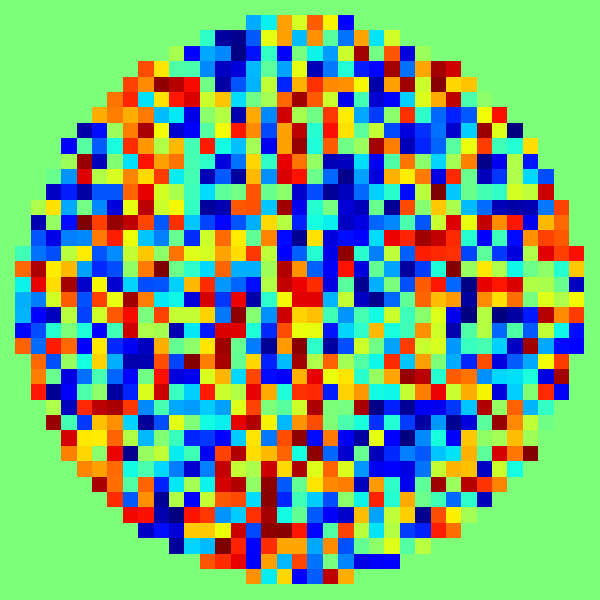
\includegraphics[width=2.45cm]{domain1}};
\end{scope}
\shade[ball color=white, opacity=0.15] (1.7, 4.95) circle (1.15);
\draw[darktext!35, thin] (1.7, 4.95) circle (1.15);

\node[darktext, font=\sffamily\bfseries\small] at ({\cw/2}, 4.95) {$\cdots$};

\begin{scope}
  \clip (4.6, 4.95) circle (1.15);
  \node[inner sep=0pt] at (4.6, 4.95) {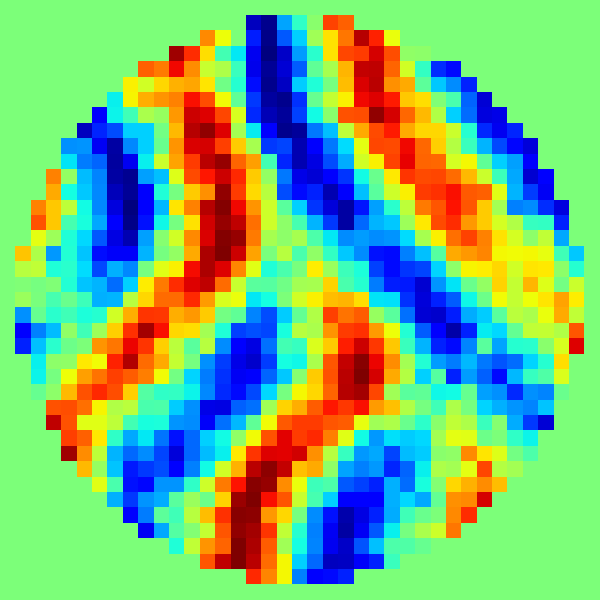
\includegraphics[width=2.45cm]{domain2}};
\end{scope}
\shade[ball color=white, opacity=0.15] (4.6, 4.95) circle (1.15);
\draw[darktext!35, thin] (4.6, 4.95) circle (1.15);

% Colorbar (m_z)
\def\cbY{3.4}
\def\cbXstart{1.15}
\def\cbLen{4.0}
\def\cbH{0.22}

\node[darktext, font=\sffamily\small\itshape] at ({\cbXstart+\cbLen/2}, {\cbY+0.45}) {$m_z$};

\shade[left color=blue!85, right color=white]
  (\cbXstart, \cbY) rectangle ({\cbXstart+\cbLen/2}, {\cbY+\cbH});
\shade[left color=white, right color=red!85]
  ({\cbXstart+\cbLen/2}, \cbY) rectangle ({\cbXstart+\cbLen}, {\cbY+\cbH});
\draw[darktext!40, very thin]
  (\cbXstart, \cbY) rectangle ({\cbXstart+\cbLen}, {\cbY+\cbH});

\node[darktext, font=\sffamily\scriptsize] at (\cbXstart, {\cbY-0.18}) {$-1$};
\node[darktext, font=\sffamily\scriptsize] at ({\cbXstart+\cbLen/2}, {\cbY-0.18}) {$0$};
\node[darktext, font=\sffamily\scriptsize] at ({\cbXstart+\cbLen}, {\cbY-0.18}) {$1$};

% Bottom text
\node[darktext, font=\sffamily\small, text width=5.8cm, align=center]
  at ({\cw/2}, 2.4) {Dataset covering diverse Hamiltonian configurations};

\node[draw=col1border, fill=white, rounded corners=3pt,
      font=\sffamily\small, inner sep=5pt, text width=5cm, align=center]
  at ({\cw/2}, 1) {
    \textbf{Hamiltonian parameters}\\[3pt]
    $\tilde{J}_1,\;\tilde{J}_2,\;\tilde{J}_3,\;\tilde{J}_4$\\[2pt]
    $\tilde{K}_{\!an1},\;\tilde{K}_{\!anS},\;\tilde{H}_{ex},\;\tilde{K}_{\!DM}$
  };
\end{scope}

% ============================================================
%  COLUMN 2: INVERSE ESTIMATION
% ============================================================
\begin{scope}[shift={($(C2)+(0.35, 0)$)}]
\def\cw{6.3}

\node[darktext, font=\sffamily\small, text width=6.0cm, align=center]
  at ({\cw/2}, 9.25) {Predict Hamiltonian parameters\\from 2D textures};

% Dataset sphere
\begin{scope}
  \clip ({\cw/2}, 7.85) circle (0.9);
  \node[inner sep=0pt] at ({\cw/2}, 7.85) {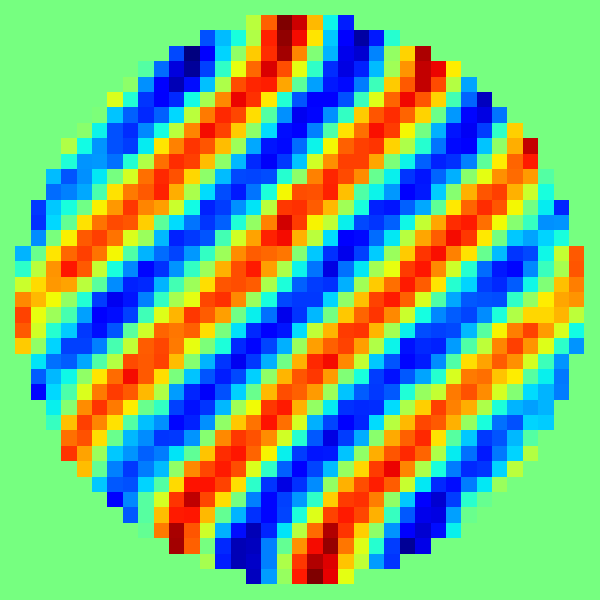
\includegraphics[width=2.1cm]{domain3}};
\end{scope}
\shade[ball color=white, opacity=0.15] ({\cw/2}, 7.85) circle (0.9);
\draw[darktext!35, thin] ({\cw/2}, 7.85) circle (0.9);

\node[font=\sffamily\small\bfseries, darktext] at ({\cw/2 + 1.7}, 7.85) {Dataset};

% Arrow down
\draw[-{Stealth[length=1mm, width=1mm]}, darktext!70, thick]
  ({\cw/2}, 6.75) -- ({\cw/2}, 6.35);

% DL Model block (3D layered)
\def\dX{0.5}
\def\dY{0.4}
\def\pW{0.2}
\def\pGap{0.15}
\def\pBot{4.0}

\pgfmathsetmacro{\startX}{3.15 - 0.5*(4*\pW + 3*\pGap)}

% Layer 1
\pgfmathsetmacro{\pOneX}{\startX}
\def\pOneH{1.7}
\fill[cnnblue1, draw=cnnblue1!35!black, thin]
  (\pOneX, \pBot) rectangle +(\pW, \pOneH);
\fill[cnnblue1!55, draw=cnnblue1!35!black, thin]
  (\pOneX, {\pBot+\pOneH}) -- +(\dX, \dY) -- +(\pW+\dX, \dY) -- +(\pW, 0) -- cycle;
\fill[cnnblue1!75, draw=cnnblue1!35!black, thin]
  ({\pOneX+\pW}, \pBot) -- +(\dX, \dY) -- +({\dX}, {\pOneH+\dY}) -- +(0, \pOneH) -- cycle;

% Layer 2
\pgfmathsetmacro{\pTwoX}{\startX + \pW + \pGap}
\def\pTwoH{1.45}
\pgfmathsetmacro{\pTwoBot}{\pBot + \pOneH/2 - \pTwoH/2}
\fill[cnnblue2, draw=cnnblue2!35!black, thin]
  (\pTwoX, \pTwoBot) rectangle +(\pW, \pTwoH);
\fill[cnnblue2!55, draw=cnnblue2!35!black, thin]
  (\pTwoX, {\pTwoBot+\pTwoH}) -- +(\dX, \dY) -- +(\pW+\dX, \dY) -- +(\pW, 0) -- cycle;
\fill[cnnblue2!75, draw=cnnblue2!35!black, thin]
  ({\pTwoX+\pW}, \pTwoBot) -- +(\dX, \dY) -- +({\dX}, {\pTwoH+\dY}) -- +(0, \pTwoH) -- cycle;

% Layer 3
\pgfmathsetmacro{\pThreeX}{\startX + 2*(\pW + \pGap)}
\def\pThreeH{1.15}
\pgfmathsetmacro{\pThreeBot}{\pBot + \pOneH/2 - \pThreeH/2}
\fill[cnnblue3, draw=cnnblue3!35!black, thin]
  (\pThreeX, \pThreeBot) rectangle +(\pW, \pThreeH);
\fill[cnnblue3!55, draw=cnnblue3!35!black, thin]
  (\pThreeX, {\pThreeBot+\pThreeH}) -- +(\dX, \dY) -- +(\pW+\dX, \dY) -- +(\pW, 0) -- cycle;
\fill[cnnblue3!75, draw=cnnblue3!35!black, thin]
  ({\pThreeX+\pW}, \pThreeBot) -- +(\dX, \dY) -- +({\dX}, {\pThreeH+\dY}) -- +(0, \pThreeH) -- cycle;

% Layer 4
\pgfmathsetmacro{\pFourX}{\startX + 3*(\pW + \pGap)}
\def\pFourH{0.85}
\pgfmathsetmacro{\pFourBot}{\pBot + \pOneH/2 - \pFourH/2}
\fill[cnngreen, draw=cnngreen!35!black, thin]
  (\pFourX, \pFourBot) rectangle +(\pW, \pFourH);
\fill[cnngreen!55, draw=cnngreen!35!black, thin]
  (\pFourX, {\pFourBot+\pFourH}) -- +(\dX, \dY) -- +(\pW+\dX, \dY) -- +(\pW, 0) -- cycle;
\fill[cnngreen!75, draw=cnngreen!35!black, thin]
  ({\pFourX+\pW}, \pFourBot) -- +(\dX, \dY) -- +({\dX}, {\pFourH+\dY}) -- +(0, \pFourH) -- cycle;

\node[font=\sffamily\small\bfseries, darktext] at (1.5, 5.2) {DL Model};

% Arrow down
\draw[-{Stealth[length=1mm, width=1mm]}, darktext!70, thick]
  ({\cw/2}, 4.0) -- ({\cw/2}, 3.65);

% Predicted Parameters label
\node[font=\sffamily\small\bfseries, darktext, text width=2.2cm, align=center]
  at ({\cw/2 + 2.2}, 2.0) {Predicted\\Parameters};

% Regression plot
\node[inner sep=0pt] at ({\cw/2 - 0.4}, 1.8) {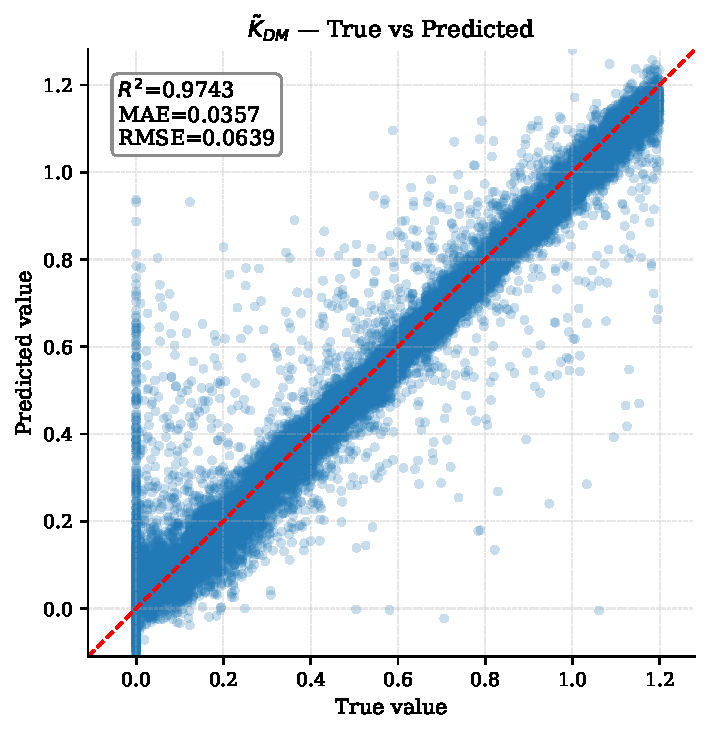
\includegraphics[width=3cm]{regression}};

\end{scope}

% ============================================================
%  COLUMN 3: INTERPRETABILITY
% ============================================================
\begin{scope}[shift={($(C3)+(0.35, 0)$)}]
\def\cw{6.3}

\node[darktext, font=\sffamily\small, text width=\cw cm, align=center]
  at ({\cw/2}, 8.9) {Visually and quantitatively connect\\ latent behavior with physical phenomena};

% a) Latent space and physical insight
\node[font=\sffamily\footnotesize\bfseries, darktext] at ({\cw/2}, 7.5)
  {a) Latent space and physical insight};

\node[inner sep=0pt] at ({\cw/2}, 5) {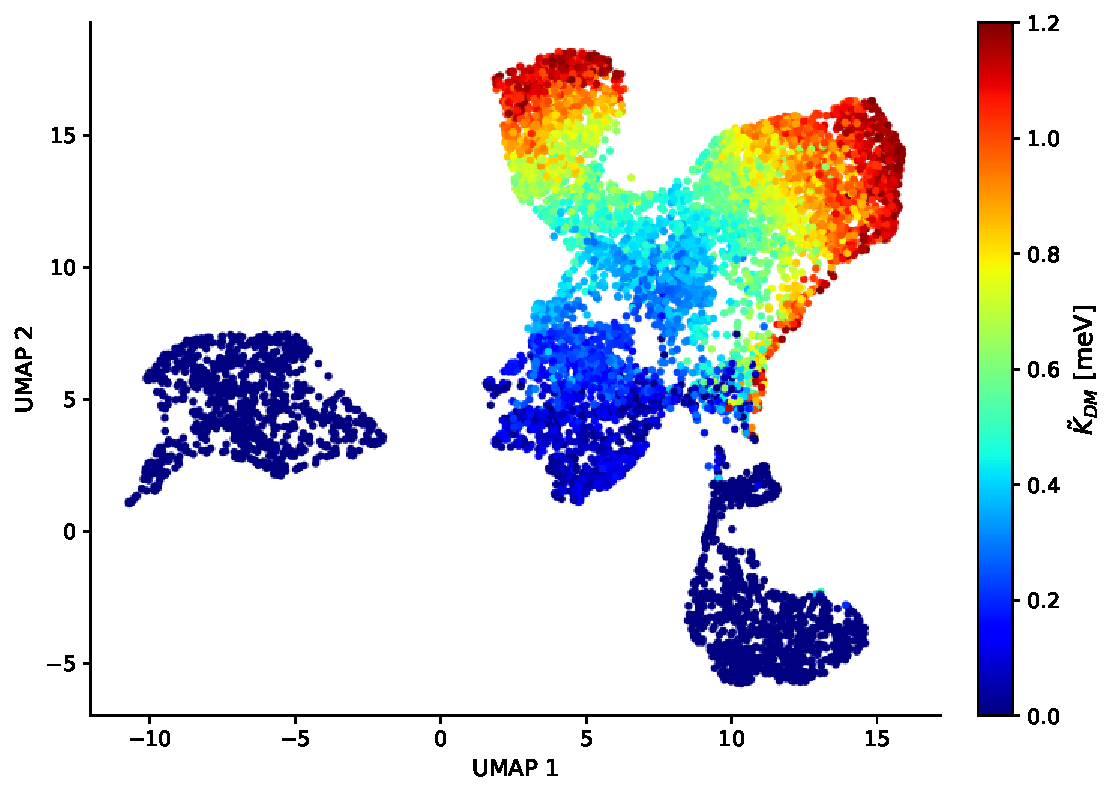
\includegraphics[width=6.0cm]{UMAP}};

% b) RAMs
\node[font=\sffamily\footnotesize\bfseries, darktext] at ({\cw/2}, 2.1)
  {b) Regression Activation Maps (RAMs)};

\node[inner sep=0pt] at ({\cw/2}, 1.2) {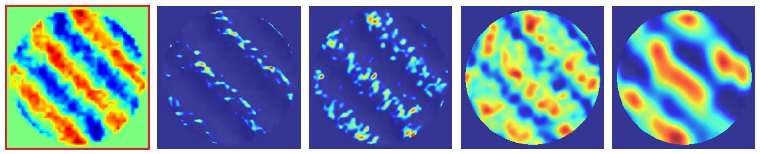
\includegraphics[width=6.0cm]{RAMsg}};

\end{scope}

\end{tikzpicture}
